% 注意事项:编译两次,以确保目录、页码完整显示

\def\allfiles{}

\documentclass[14pt,a4paper,UTF8,twoside]{article}

% Formatting Packages ——————————————————————————————————————
\usepackage{multicol}
\usepackage{multirow}
\usepackage{enumitem}
\usepackage{indentfirst}
\usepackage[toc]{multitoc}

% Math & Physics Packages ————————————————————————————
\usepackage{amsmath, amsthm, amsfonts, amssymb}
\usepackage{setspace}
\usepackage{physics}
\usepackage{cancel}
\usepackage{nicefrac}
\usepackage{unicode-math} % 允许数学公式使用特定字体

% Image-related Packages —————————————————————————————
\usepackage{float} % 浮动体环境
\usepackage{subcaption} % 子图包
\usepackage{graphics, graphicx}
\usepackage{tikz, tikz-qtree}
\usetikzlibrary{arrows.meta}
\usetikzlibrary{shapes.geometric, arrows}
\tikzstyle{node_style} = [rectangle, rounded corners, draw, align=center, text width=3cm, minimum height=0.65cm]
\tikzstyle{arrow_style} = [thick, ->, >=stealth]

\usepackage{pgfplots}
\pgfplotsset{compat=1.18}
\usepackage{xcolor}
\usepackage{fourier-orns}
\usepackage{lipsum}

% Colour Palette ——————————————————————————————————————
\definecolor{merah}{HTML}{F4564E}
\definecolor{merahtua}{HTML}{89313E}
\definecolor{biru}{HTML}{60BBE5}
\definecolor{birutua}{HTML}{412F66}
\definecolor{hijau}{HTML}{59CC78}
\definecolor{hijautua}{HTML}{366D5B}
\definecolor{kuning}{HTML}{FFD56B}
\definecolor{jingga}{HTML}{FBA15F}
\definecolor{ungu}{HTML}{8C5FBF}
\definecolor{lavender}{HTML}{CBA5E8}
\definecolor{merjamb}{HTML}{FFB6E0}
\definecolor{mygray}{HTML}{E6E6E6}
\definecolor{mygreen}{rgb}{0,0.6,0}
\definecolor{mymauve}{rgb}{0.58,0,0.82}

% Theorems ————————————————————————————————————————————
\usepackage{tcolorbox}
\usepackage{changepage}
\tcbuselibrary{skins,breakable,theorems}

\newcounter{hitung}
\setcounter{hitung}{\thesection}

\makeatletter
	% Proof 证明如下
	\def\tcb@theo@widetitle#1#2#3{\hbox to \textwidth{\textsc{\large#1}\normalsize\space#3\hfil(#2)}}
	\tcbset{
		theorem style/theorem wide name and number/.code={ \let\tcb@theo@title=\tcb@theo@widetitle},
		proofbox/.style={skin=enhancedmiddle,breakable,parbox=false,boxrule=0mm,
			check odd page, toggle left and right, colframe=black!20!white!92!hijau,
			leftrule=8pt, rightrule=0mm, boxsep=0mm,arc=0mm, outer arc=0mm,
			left=3mm,right=3mm,top=0mm,bottom=0mm, toptitle=0mm,
			bottomtitle=0mm,colback=gray!3!white!98!biru, before skip=8pt, after skip=8pt,
			before={\par\vskip-2pt},after={\par\smallbreak},
		},
	}
	\newtcolorbox{ProofBox}{proofbox}
	\makeatother
	
	\let\realproof\proof
	\let\realendproof\endproof
	\renewenvironment{proof}[1][Prove:]{\ProofBox\strut\textsc{#1}\space}{\endProofBox}
        \AtEndEnvironment{proof}{\null\hfill$\blacksquare$}
        % Definition 定义环境
	\newtcbtheorem[use counter=hitung, number within=section]{dfn}{定义}
	{theorem style=theorem wide name and number,breakable,enhanced,arc=3.5mm,outer arc=3.5mm,
		boxrule=0pt,toprule=1pt,leftrule=0pt,bottomrule=1pt, rightrule=0pt,left=0.2cm,right=0.2cm,
		titlerule=0.5em,toptitle=0.1cm,bottomtitle=-0.1cm,top=0.2cm,
		colframe=white!10!biru,
		colback=white!90!biru,
		coltitle=white,
		shadow={1.3mm}{-1.3mm}{0mm}{gray!50!white}, % 添加阴影
        coltext=birutua!60!gray, title style={white!10!biru}, rbefoe skip=8pt, after skip=8pt,
		fonttitle=\bfseries,fontupper=\normalsize}{dfn}

	% 答题卡
	\newtcbtheorem[use counter=hitung, number within=section]{ans}{解答}
	{theorem style=theorem wide name and number,breakable,enhanced,arc=3.5mm,outer arc=3.5mm,
		boxrule=0pt,toprule=1pt,leftrule=0pt,bottomrule=1pt, rightrule=0pt,left=0.2cm,right=0.2cm,
		titlerule=0.5em,toptitle=0.1cm,bottomtitle=-0.1cm,top=0.2cm,
		colframe=white!10!biru,
		colback=white!90!biru,
		coltitle=white,
		shadow={1.3mm}{-1.3mm}{0mm}{gray!50!white}, % 添加阴影
        coltext=birutua!60!gray, title style={white!10!biru}, before skip=8pt, after skip=8pt,
		fonttitle=\bfseries,fontupper=\normalsize}{ans}

	% Axiom
	\newtcbtheorem[use counter=hitung, number within=section]{axm}{公理}
	{theorem style=theorem wide name and number,breakable,enhanced,arc=3.5mm,outer arc=3.5mm,
		boxrule=0pt,toprule=1pt,leftrule=0pt,bottomrule=1pt, rightrule=0pt,left=0.2cm,right=0.2cm,
		titlerule=0.5em,toptitle=0.1cm,bottomtitle=-0.1cm,top=0.2cm,
		colframe=white!10!biru,colback=white!90!biru,coltitle=white,
		shadow={1.3mm}{-1.3mm}{0mm}{gray!50!white!90}, % 添加阴影
        coltext=birutua!60!gray,title style={white!10!biru},before skip=8pt, after skip=8pt,
		fonttitle=\bfseries,fontupper=\normalsize}{axm}
 
	% Theorem
	\newtcbtheorem[use counter=hitung, number within=section]{thm}{定理}
	{theorem style=theorem wide name and number,breakable,enhanced,arc=3.5mm,outer arc=3.5mm,
		boxrule=0pt,toprule=1pt,leftrule=0pt,bottomrule=1pt, rightrule=0pt,left=0.2cm,right=0.2cm,
		titlerule=0.5em,toptitle=0.1cm,bottomtitle=-0.1cm,top=0.2cm,
		colframe=white!10!merah,colback=white!75!pink,coltitle=white, coltext=merahtua!80!merah,
		shadow={1.3mm}{-1.3mm}{0mm}{gray!50!white!90}, % 添加阴影
		title style={white!10!merah}, before skip=8pt, after skip=8pt,
		fonttitle=\bfseries,fontupper=\normalsize}{thm}
	
	% Proposition
	\newtcbtheorem[use counter=hitung, number within=section]{prp}{命题}
	{theorem style=theorem wide name and number,breakable,enhanced,arc=3.5mm,outer arc=3.5mm,
		boxrule=0pt,toprule=1pt,leftrule=0pt,bottomrule=1pt, rightrule=0pt,left=0.2cm,right=0.2cm,
		titlerule=0.5em,toptitle=0.1cm,bottomtitle=-0.1cm,top=0.2cm,
		colframe=white!10!hijau,colback=white!90!hijau,coltitle=white, coltext=hijautua!80!brown,
		shadow={1.3mm}{-1.3mm}{0mm}{gray!50!white}, % 添加阴影
		title style={white!10!hijau}, before skip=8pt, after skip=8pt,
		fonttitle=\bfseries,fontupper=\normalsize}{prp}


	% Example
	\newtcolorbox[use counter=hitung, number within=section]{cth}[1][]{breakable,
		colframe=white!10!jingga, coltitle=white!90!jingga, colback=white!85!jingga, coltext=black!10!brown!50!jingga, colbacktitle=white!10!jingga, enhanced, fonttitle=\bfseries,fontupper=\normalsize, attach boxed title to top left={yshift=-2mm}, before skip=8pt, after skip=8pt,
		title=Contoh~\thetcbcounter \ \ #1}

	% Catatan/Note
	\newtcolorbox{ctt}[1][]{enhanced, 
		left=4.1mm, borderline west={8pt}{0pt}{white!10!kuning}, 
		before skip=6pt, after skip=6pt, 
		colback=white!85!kuning, colframe= white!85!kuning, coltitle=orange!60!kuning!25!brown, coltext=orange!60!kuning!25!brown,
		fonttitle=\bfseries,fontupper=\normalsize, before skip=8pt, after skip=8pt,
		title=\underline{Catatan}  #1}
	
	% Komentar/Remark
	\newtcolorbox{rmr}[1][]{
		,arc=0mm,outer arc=0mm,
		boxrule=0pt,toprule=1pt,leftrule=0pt,bottomrule=5pt, rightrule=0pt,left=0.2cm,right=0.2cm,
		titlerule=0.5em,toptitle=0.1cm,bottomtitle=-0.1cm,top=0.2cm,
		colframe=white!10!kuning,colback=white!85!kuning,coltitle=white, coltext=orange!60!kuning,
		fonttitle=\bfseries,fontupper=\normalsize, before skip=8pt, after skip=8pt,
		title=Komentar  #1}

\usepackage{booktabs} % 表格库
\usepackage{titlesec} % 标题库
\usepackage{fancyhdr} % 页眉页脚库
\usepackage[sorting=none]{biblatex}
\usepackage{array}
\addbibresource{references.bib} % 指定你的.bib文件名称

\date{} % 留空,以让编译时去除日期

%———————————————注意事项—————————————————%

% 1、如果编译显示失败,但没有错误信息,就是 filename.pdf 正在被占用
% 2、在文件夹中的终端使用 Windows > xelatex filename.tex 也可编译

%—————————————华东师范大学———————————————%

% 论文制作时须加页眉,页眉从中文摘要开始至论文末
% 偶数页码内容为:华东师范大学硕士学位论文,奇数页码内容为学位论文题目

%————————定义 \section 的标题样式————————%

% 注意:\chapter 等命令,内部使用的是 \thispagestyle{plain} 的排版格式
% 若需要自己加上页眉,实际是在用 \thispagestyle{fancy} 的排版格式
% 加上下面这一段指令,就能够让 \section 也使用 fancy 的排版格式
% 本质就是让目录、第一页也能够显示页眉、页脚

\fancypagestyle{plain}{
  \pagestyle{fancy}
}

\title{华东师范大学软件学院实验报告} % 模板
\titleformat{\section}
    {\normalfont\bfseries\Large} % 字体大小、字体系列(\bfseries 为加粗)
    {\thesection}{1em}{}

% ———————————设置章节的中文格式———————————%
\renewcommand\thesection{\chinese{section} \hspace{0pt}}
\renewcommand\thesubsection{\arabic{subsection} \hspace{0pt}}
% \renewcommand\thesubsubsection{\alph{subsubsection} \hspace{0pt}} % 字母编号
% \hspace{0pt} 是为了确保在章节编号和章节题目之间不要有空格,使得排版更为美观
    
%—————————————页面基础设置———————————————%

\usepackage{geometry}
\geometry{left=10mm, right=10mm, top=20mm, bottom=20mm}

%————————————设置页眉、页脚——————————————%

\pagestyle{fancy} % 设置 plain style 的属性

% 设置页眉

\fancyhead[RE]{\leftmark} % Right Even 偶数页右侧显示章名 \leftmark 最高级别章名
\fancyhead[LO]{\rightmark} % Left Odd 奇数页左侧显示节名 \rightmark 第二级别节名
\fancyhead[C]{华东师范大学软件学院实验报告} % Center 居中显示
\fancyhead[LE,RO]{~\thepage~} % 在偶数页的左侧,奇数页的右侧显示页码
\renewcommand{\headrulewidth}{1.2pt} % 页眉与正文之间的水平线粗细

% 设置页脚:在每页的右下脚以斜体显示书名

\fancyfoot[RO,RE]{\it Lab Report By \LaTeX} % 使用意大利斜体显示
\renewcommand{\footrulewidth}{0.5pt} % 页脚水平线宽度

%——————设置页码:在底部居中显示页码———————%

\usepackage{lastpage} % 页码数库
\pagestyle{fancy}
\fancyfoot[C]{\kaishu 第 \thepage 页 \ 共 \pageref{LastPage} 页} % LastPage 需要二次编译以获取总页数

%——————————————代码块设置———————————————%

\usepackage{listings} % 代码块包
\lstset {
    backgroundcolor=\color{white},   % choose the background color; you must add \usepackage{color} or \usepackage{xcolor}
    basicstyle=\footnotesize,        % the size of the fonts that are used for the code
    breakatwhitespace=false,         % sets if automatic breaks should only happen at whitespace
    breaklines=true,                 % sets automatic line breaking
    captionpos=bl,                   % sets the caption-position to bottom
    commentstyle=\color{mygreen},    % comment style
    deletekeywords={...},            % if you want to delete keywords from the given language
    escapeinside={\%*}{*},           % if you want to add LaTeX within your code
    extendedchars=true,              % lets you use non-ASCII characters; for 8-bits encodings only, does not work with UTF-8
    frame=single,                    % adds a frame around the code
    keepspaces=true,                 % keeps spaces in text, useful for keeping indentation of code (possibly needs columns=flexible)
    keywordstyle=\color{blue},       % keyword style
    % language=Python,               % the language of the code
    morekeywords={*,...},            % if you want to add more keywords to the set
    numbers=left,                    % where to put the line-numbers; possible values are (none, left, right)
    numbersep=5pt,                   % how far the line-numbers are from the code
    numberstyle=\tiny\color{mygray}, % the style that is used for the line-numbers
    rulecolor=\color{black},         % if not set, the frame-color may be changed on line-breaks within not-black text (e.g. comments (green here))
    showspaces=false,                % show spaces everywhere adding particular underscores; it overrides 'showstringspaces'
    showstringspaces=false,          % underline spaces within strings only
    showtabs=false,                  % show tabs within strings adding particular underscores
    stepnumber=1,                    % the step between two line-numbers. If it's 1, each line will be numbered
    stringstyle=\color{orange},      % string literal style
    tabsize=2,                       % sets default tabsize to 2 spaces
    % title=Python Code              % show the filename of files included with \lstinputlisting; also try caption instead of title
}

% 注释掉的部分用于后续插入代码,参数可调整,格式如下:

% 1、直接插入
% \begin{lstlisting}[language = ? , title = { ? } ]
%       Your code here.
% \end{lstlisting}

% 2、文件插入
% \lstinputlisting[language = C , title = ?.c] {filename.c}

%———————————————字体设置————————————————%

\usepackage{fontspec} % 允许设置字体
\usepackage[utf8]{inputenc}
\usepackage{ctex}
\linespread{1.2}
% \setCJKmainfont{SimSun} % 设置正文罗马族的 CJK 字体

%———————————————超链接设置——————————————%

\usepackage[hidelinks]{hyperref}
\hypersetup{
    pdfstartview=FitH, % 设置PDF文档打开时的初始视图为页面宽度适应窗口宽度(即页面水平适应)
    CJKbookmarks=true, % 用对CJK(中文、日文、韩文)字符的书签支持,确保这些字符在书签中正确显示
    bookmarksnumbered=true, % 书签带有章节编号。这对有章节编号的文档很有用
    bookmarksopen=true, % 文档打开时,书签树是展开的,方便查看所有书签
    colorlinks, % 启用彩色链接。这样,链接在PDF中会显示为彩色,而不是默认的方框
    pdfborder=001, % 设置PDF文档中链接的边框样式。001 表示链接周围没有边框,仅在单击时显示一个矩形
    linkcolor=blue, % 设置文档内部链接(如目录中的章节链接)的颜色为蓝色
    anchorcolor=blue, % 设置锚点链接(即目标在同一文档内的链接)的颜色为蓝色
    citecolor=blue, % 设置引用(如文献引用)的颜色为蓝色
}

%————————————导言区结束,进入正文部分————————————%

\begin{document}

\maketitle

\begin{center} % \extracolsep{\fill} 拉伸到页面最大宽度前,保证居中显示

  \begin{tabular*}{\textwidth}{@{\extracolsep{\fill}} l  l  l }
    \hline
    实验课程:计算机网络实践 &  年级:2023级本科  &  实验成绩: \\
    实验名称:Lab 4 ARP & 姓名:张梓卫 \\
    实验编号:(4) & 学号:10235101526 & 实验日期:2024/12/13 \\
    指导老师:刘献忠 & 组号:& 实验时间:2 课时 \\
    \hline
  \end{tabular*}

\end{center}

\tableofcontents % 目录也需要二次编译

\section{实验目的}

该实验是课程《计算机网络实践》的第四次实验,全名《ARP》,目标如下:

\begin{itemize}
    \item 1. 学会通过Wireshark获取ARP消息
    \item 2. 掌握ARP数据包结构
    \item 3. 掌握ARP数据包各字段的含义
    \item 4. 了解ARP协议适用领域    
\end{itemize}

\section{实验内容与实验步骤}

\begin{itemize}
    \item 使用管理员权限打开命令行
    \item 输入ipconfig /all,可以获得本地计算机的物理地址
    \item 输入netstat –r,可以获得本机路由表
    \item 输入arp –a,可以查看ARP cache
    \item 输入arp –d,可以清空ARP cache
    \item 启动Wireshark,在菜单栏的捕获->选项中进行设置,选择已连接的以太网,设置捕获过滤器为ARP,将混杂模式设为关闭,点击开始
    \item 清空ARP cache
\end{itemize}

\section{实验环境}

使用 Wireshark v4.2.5, Windows 11 Pro, Wget Tools 进行实验。

实验报告使用 \LaTeX 进行撰写,使用 Vim 编辑器进行文本编辑。

\section{实验过程与分析}

\subsection*{预备知识}

虽然在网络层转发分组使用的是 IP 地址,
但是最终我们还是要使用 MAC 地址在实际的网络线路上传输数据。
所以光知道目标的 IP 地址是没有用的。
ARP 就能够把 IP 地址转换为 MAC 地址。

每一台主机都有一个 ARP 缓存表,
里面记录着 IP 地址和 MAC 地址的映射关系,ARP 的职责即动态地维护该表。

查表会有两种情况:1、命中;2、缺失:(1)广播 ARP 请求;(2)更新 ARP 缓存。

ARP 报文结构,在 PPT 上如下所示:

\begin{figure}[H]
    \centering
    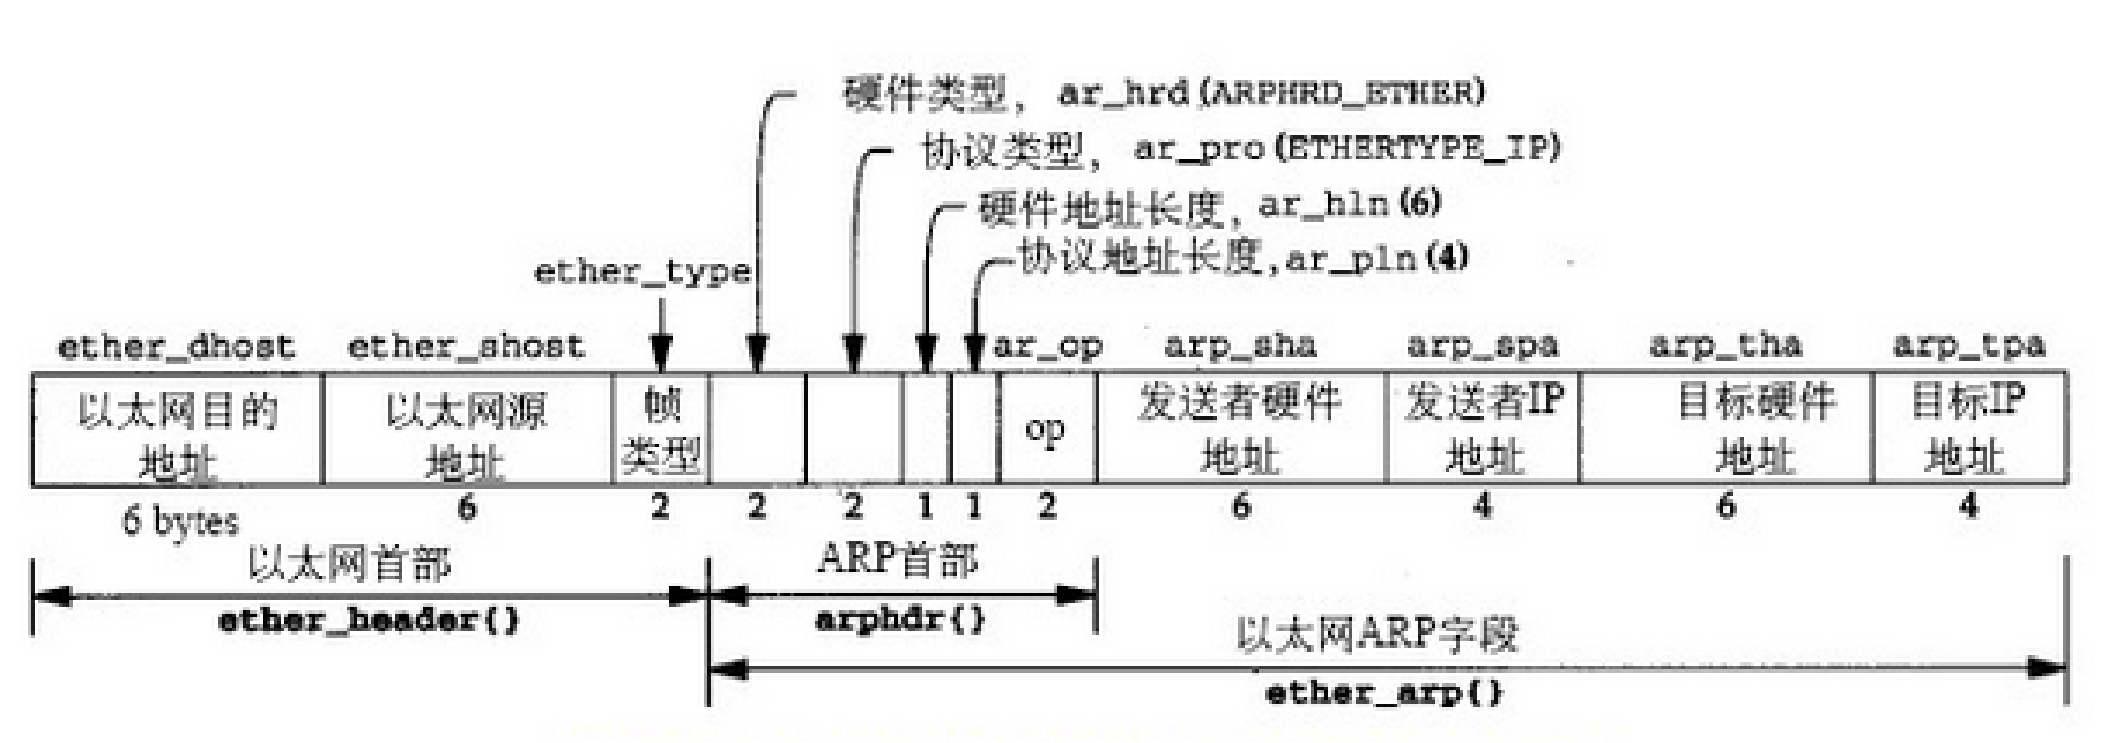
\includegraphics[width=0.6\textwidth]{lab4/arpstructure.png}
    \caption{ARP 报文结构}
\end{figure}

\subsection{Step 1: Capture a Trace}

\subsubsection{使用 ipconfig /all 查找地址}

\begin{figure}[H]
    \centering
    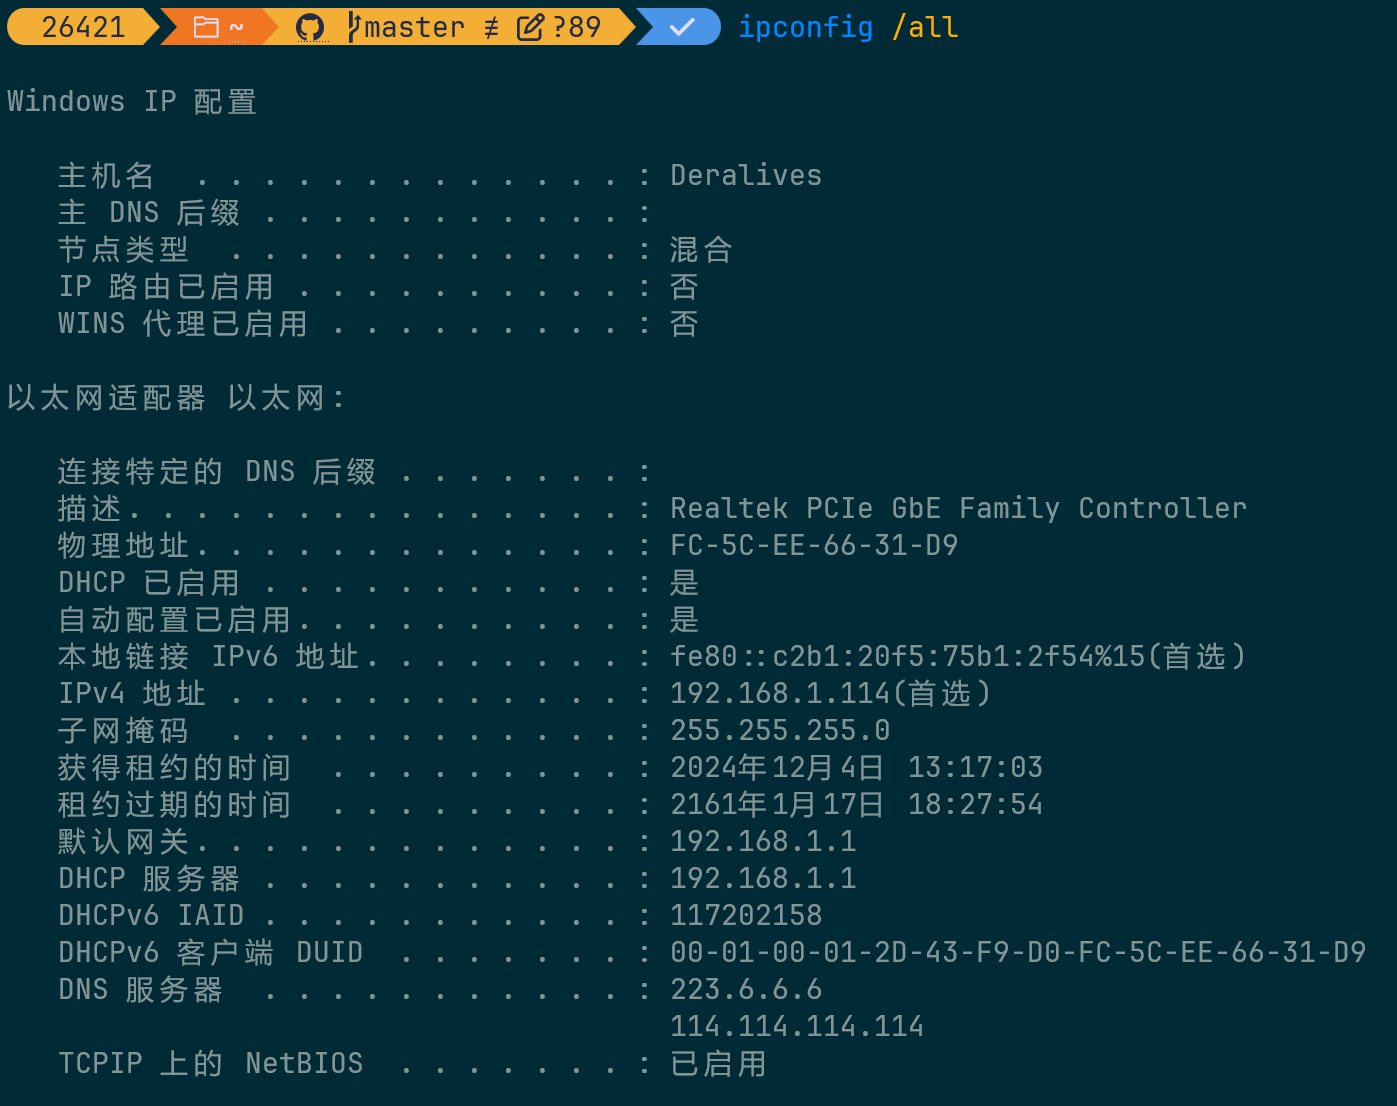
\includegraphics[width=0.5\textwidth]{lab4/ipconfigall.png}
    \caption{使用 ipconfig /all 查找地址}
\end{figure}

通过图中内容,可以分析得到,本机的 IP 地址为 192.168.1.114,MAC 地址为 \texttt{FC-5C-EE-66-31-D9}。

\subsubsection{使用 netstat 和 arp 命令}

使用 netstat -r 查看路由表。

\begin{figure}[H]
    \centering
    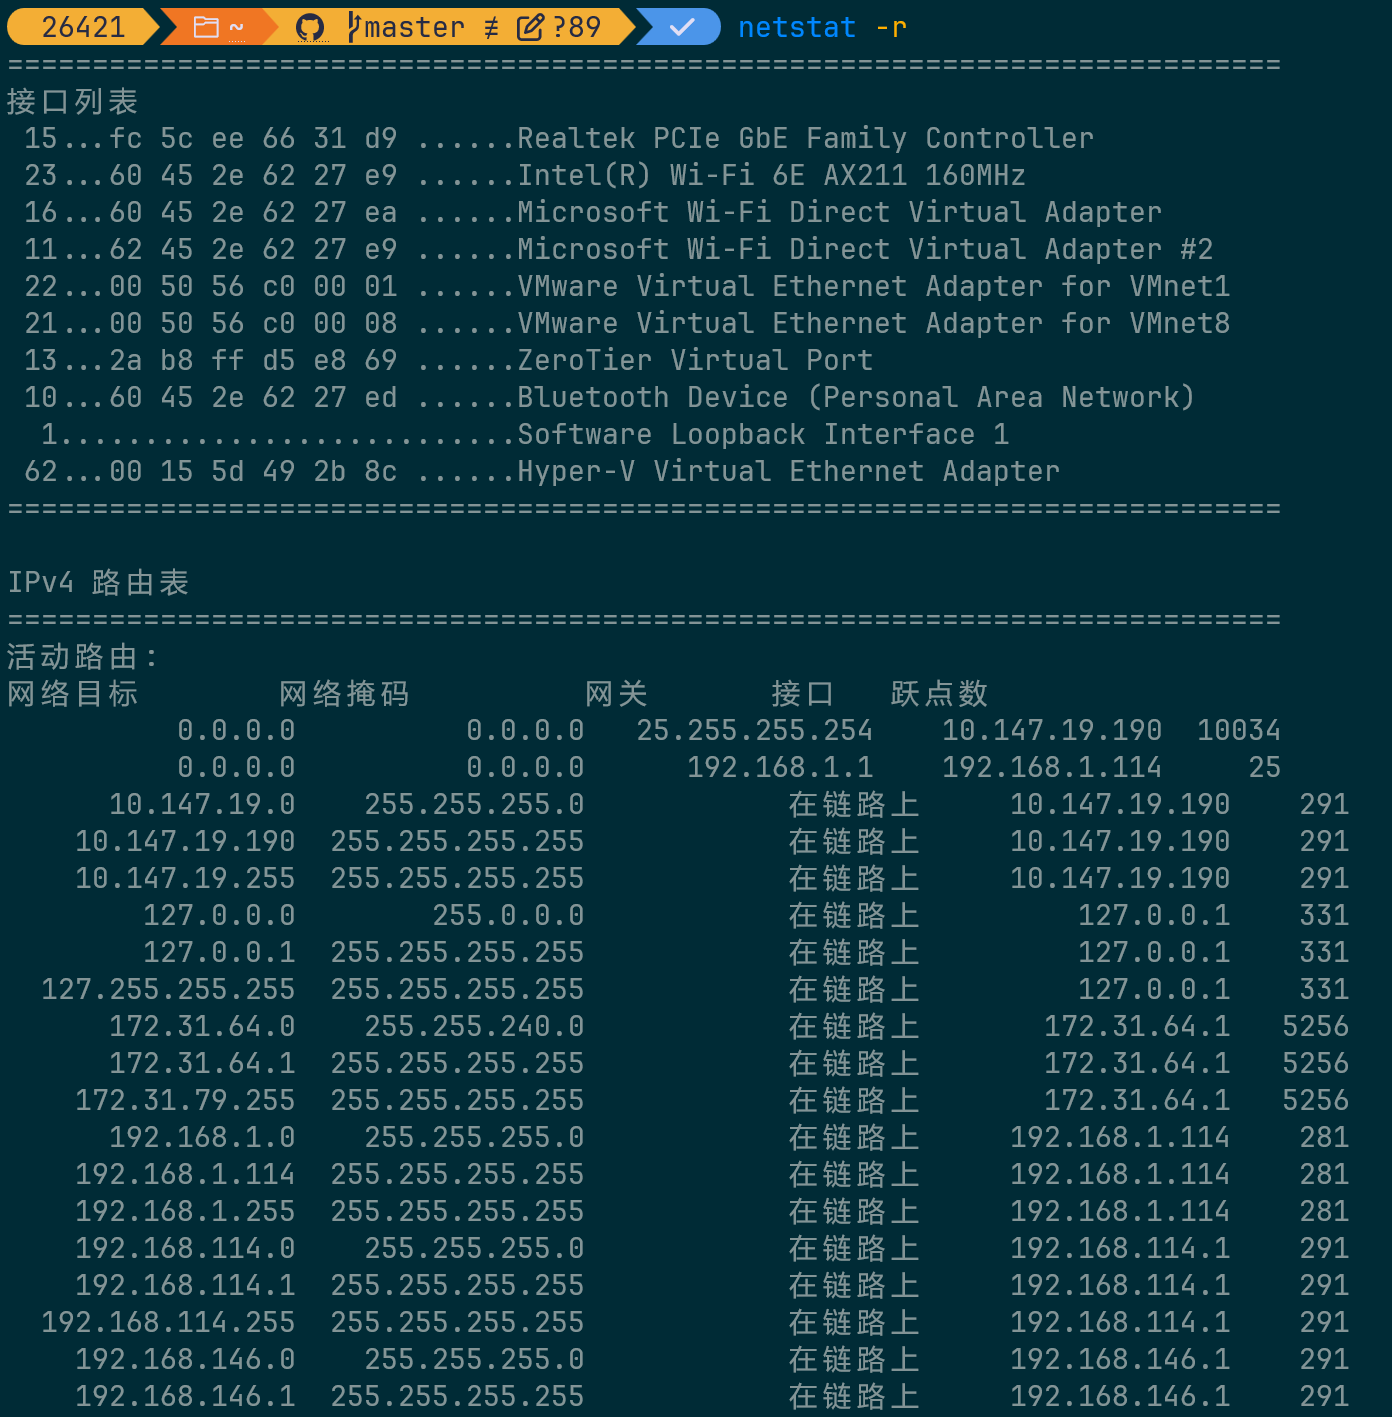
\includegraphics[width=0.5\textwidth]{lab4/routetable.png}
    \caption{使用 netstat -r 查看路由表}
\end{figure}

从图中可以看到,默认的网关 IP 为 192.168.1.1。

\subsubsection{设置 Wireshark 捕获 ARP 数据包}

将过滤器设置为 ARP,将混杂模式关闭,点击开始捕获。

\begin{figure} [H]
    \centering
    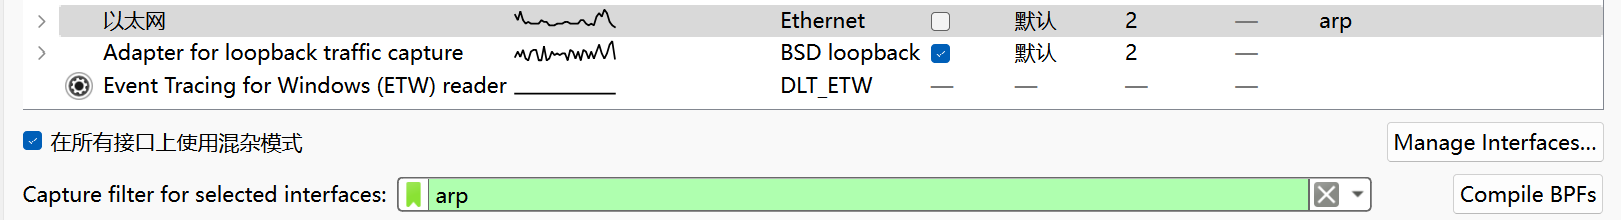
\includegraphics[width=0.8\textwidth]{lab4/arpsetting.png}
    \caption{设置 Wireshark 的过滤器}
\end{figure}

设置 rename 选项为开启:

\begin{figure}[H]
  \centering
  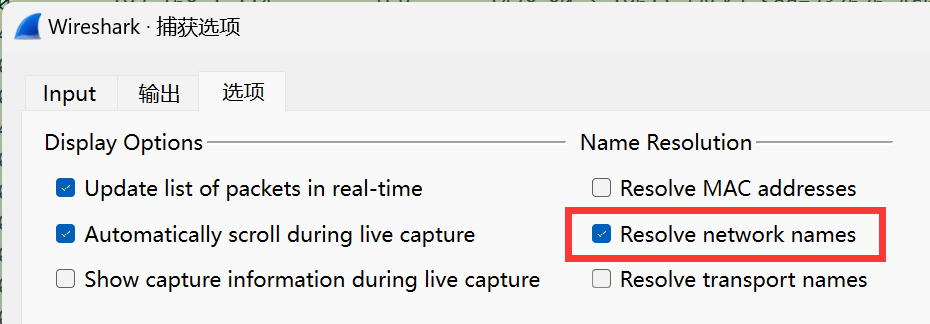
\includegraphics[width=0.4\textwidth]{lab4/rename.png}
  \caption{Wireshark Rename}
\end{figure}

在 Wireshark 中可以看到很多协议为 ARP 的数据包:

\begin{figure} [H]
    \centering
    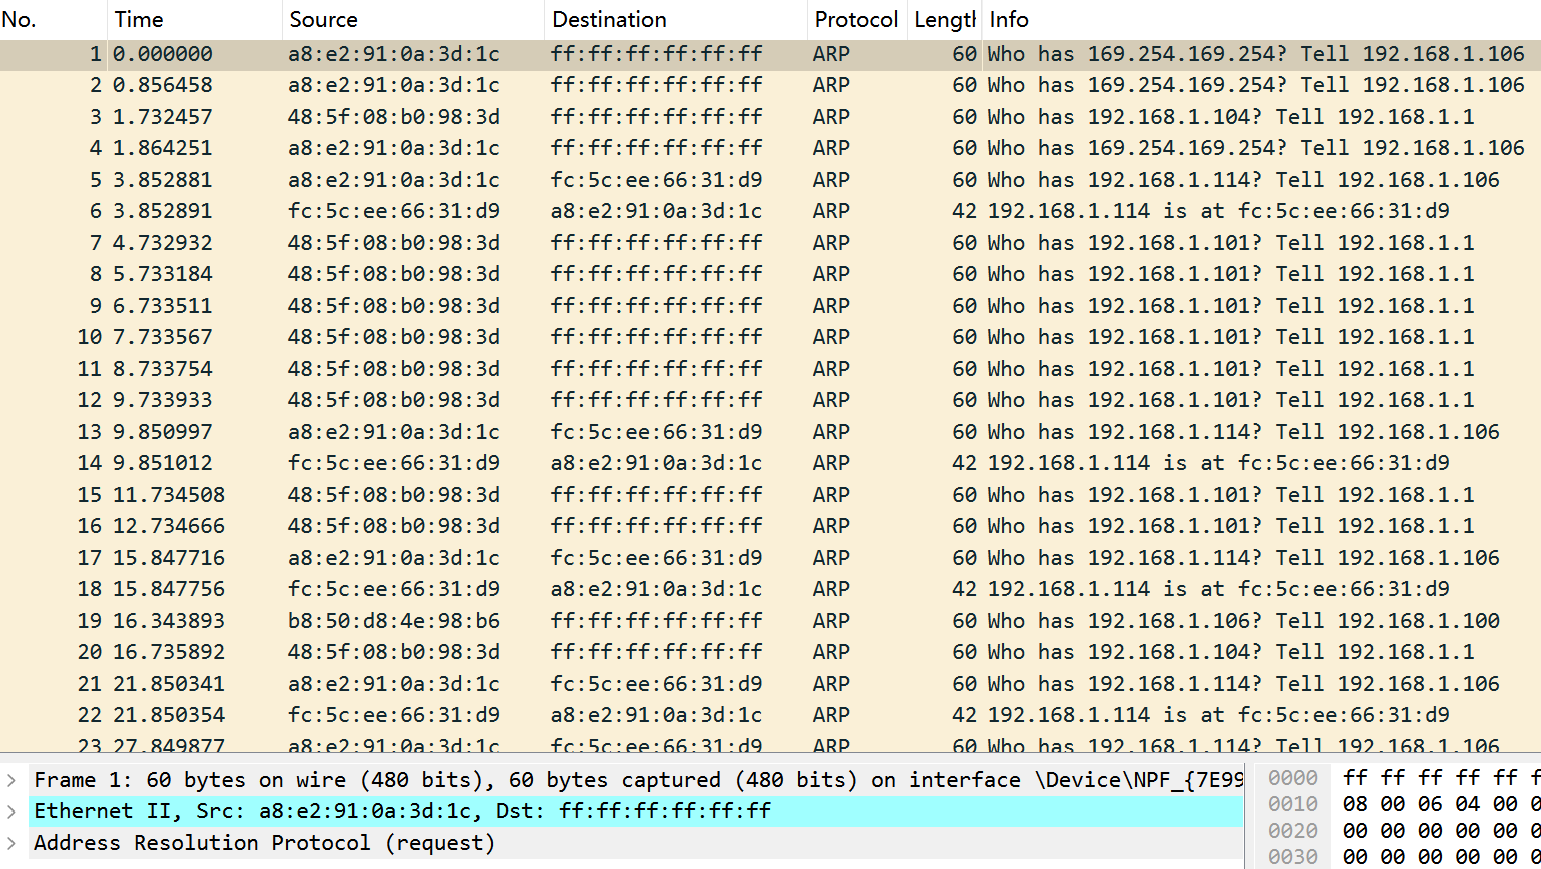
\includegraphics[width=0.8\textwidth]{lab4/arptable.png}
    \caption{Wireshark 捕获的 ARP 数据包}
\end{figure}

\subsubsection{促使 ARP 表更新}

使用管理员权限打开命令行,打开 Wireshark 开始捕获.

输入命令 \textbf{arp -d } 清空 ARP 缓存,再使用 \textbf{arp -d 192.168.1.1} 来清空和网关相关的 ARP 缓存。然后使用命令 \textbf{arp -a} 检查缓存是否清空成功。

接下来浏览任意的网页,来促使 ARP 表更新,在 Wireshark 中捕获了 ARP 报文以后,点击停止,开始分析。

我打开了 www.baidu.com,使用 Wireshark 抓包完成后,再次使用 \textbf{arp -a} 指令,可以发现 ARP 路由表发生了变化:

\begin{figure}[H]
    \centering
    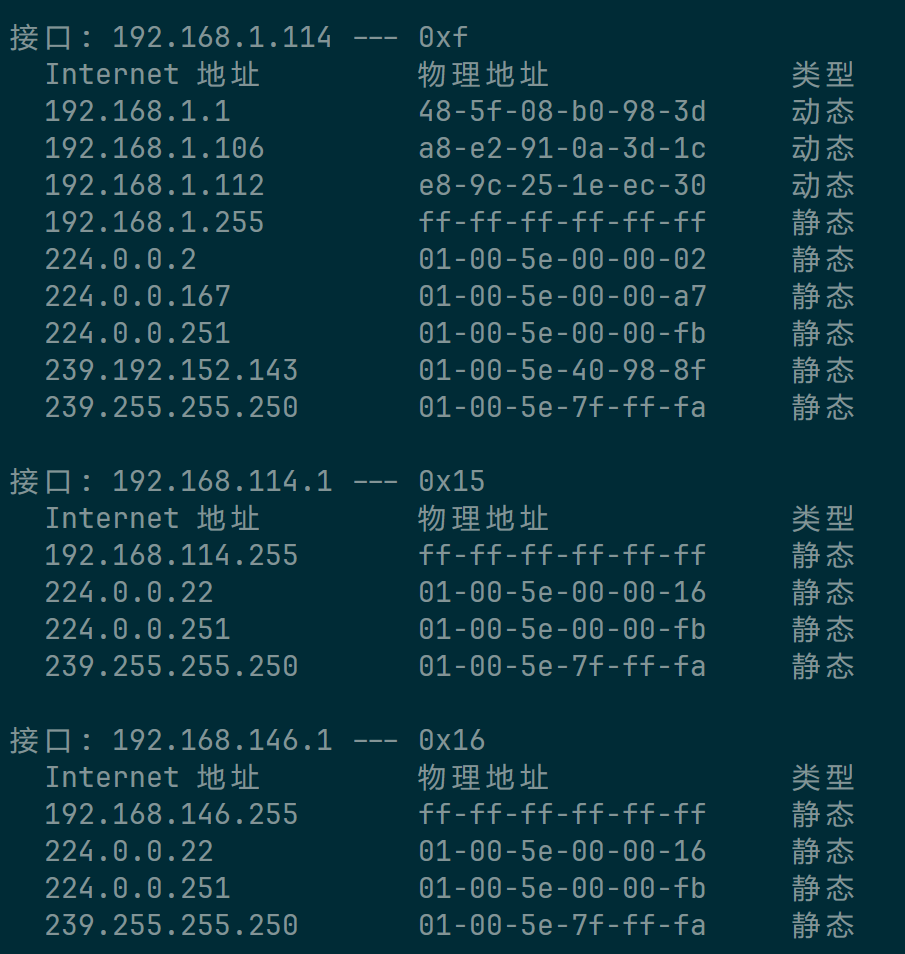
\includegraphics[width=0.4\textwidth]{lab4/arpupdate.png}
    \caption{ARP 表更新}
\end{figure}

\subsection{Step 2: Inspect The Trace}

\subsubsection{使用 MAC 地址过滤器}

在 Wireshark 中使用 \textbf{eth.addr==fc:5c:ee:66:31:d9} 来设置过滤器,以找出与自己的 MAC 地址相关的 ARP 报文。

Notice:ARP 报文包括请求报文和应答报文。

\begin{figure}[H]
    \centering
    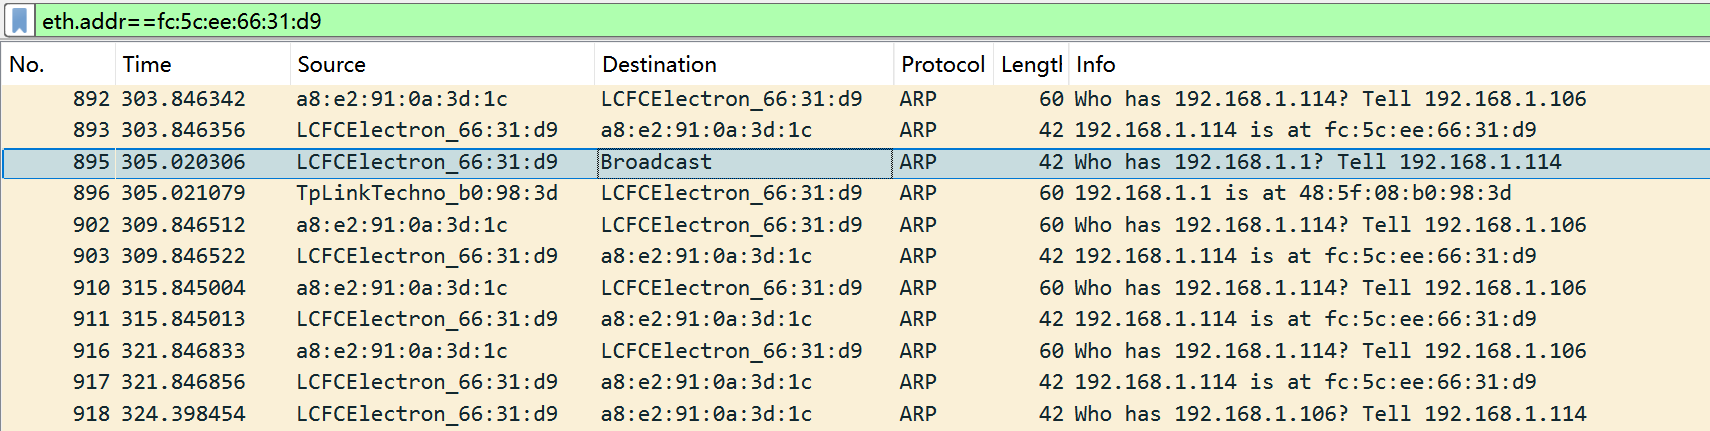
\includegraphics[width=0.8\textwidth]{lab4/macfilter.png}
    \caption{使用 MAC 地址过滤器}
\end{figure}

\subsubsection{从本机发送的包}

查看从本地发送出去的 request 帧。

\begin{figure}[H]
    \centering
    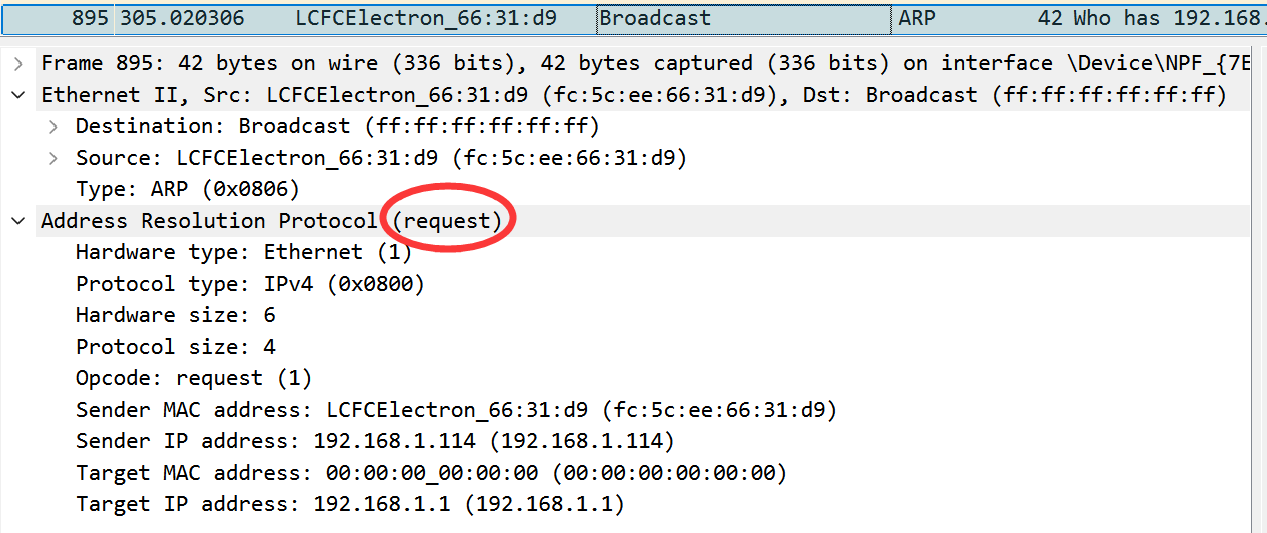
\includegraphics[width=0.65\textwidth]{lab4/request.png}
    \caption{从本机发送的 request 帧}
\end{figure}

\subsubsection{绘制 ARP 协议的结构}

我们选取刚刚获取到的 request 请求,我把 Wireshark 中显示的结构和对应的字段整合到一起,如下图所示:

\begin{figure}[H]
    \centering
    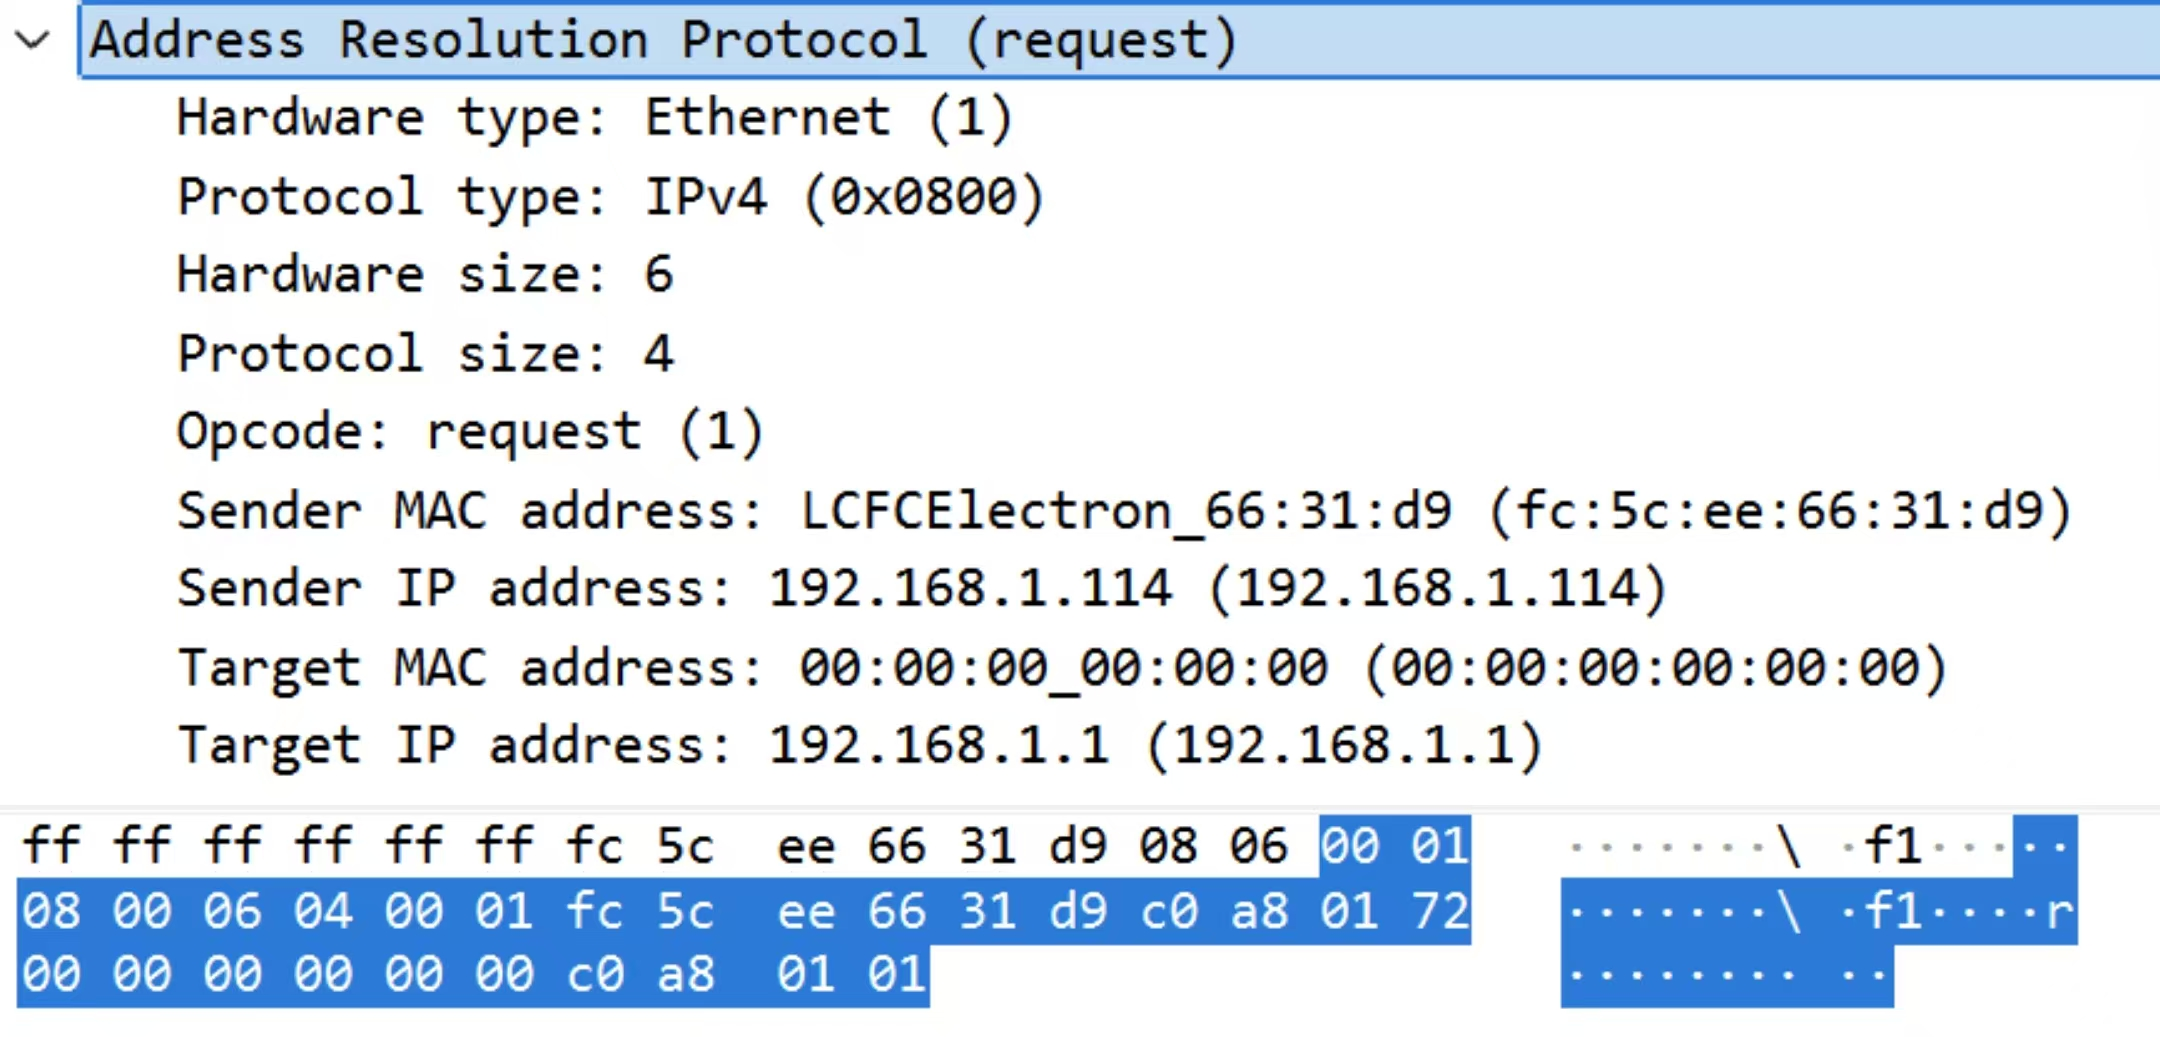
\includegraphics[width=0.4\textwidth]{lab4/example.jpg}
    \caption{Wireshark 捕获结果}
\end{figure}

然后用鼠标依次点击高亮字段,将每个字段用笔标注出来,如下图所示:

\begin{figure}[H]
    \centering
    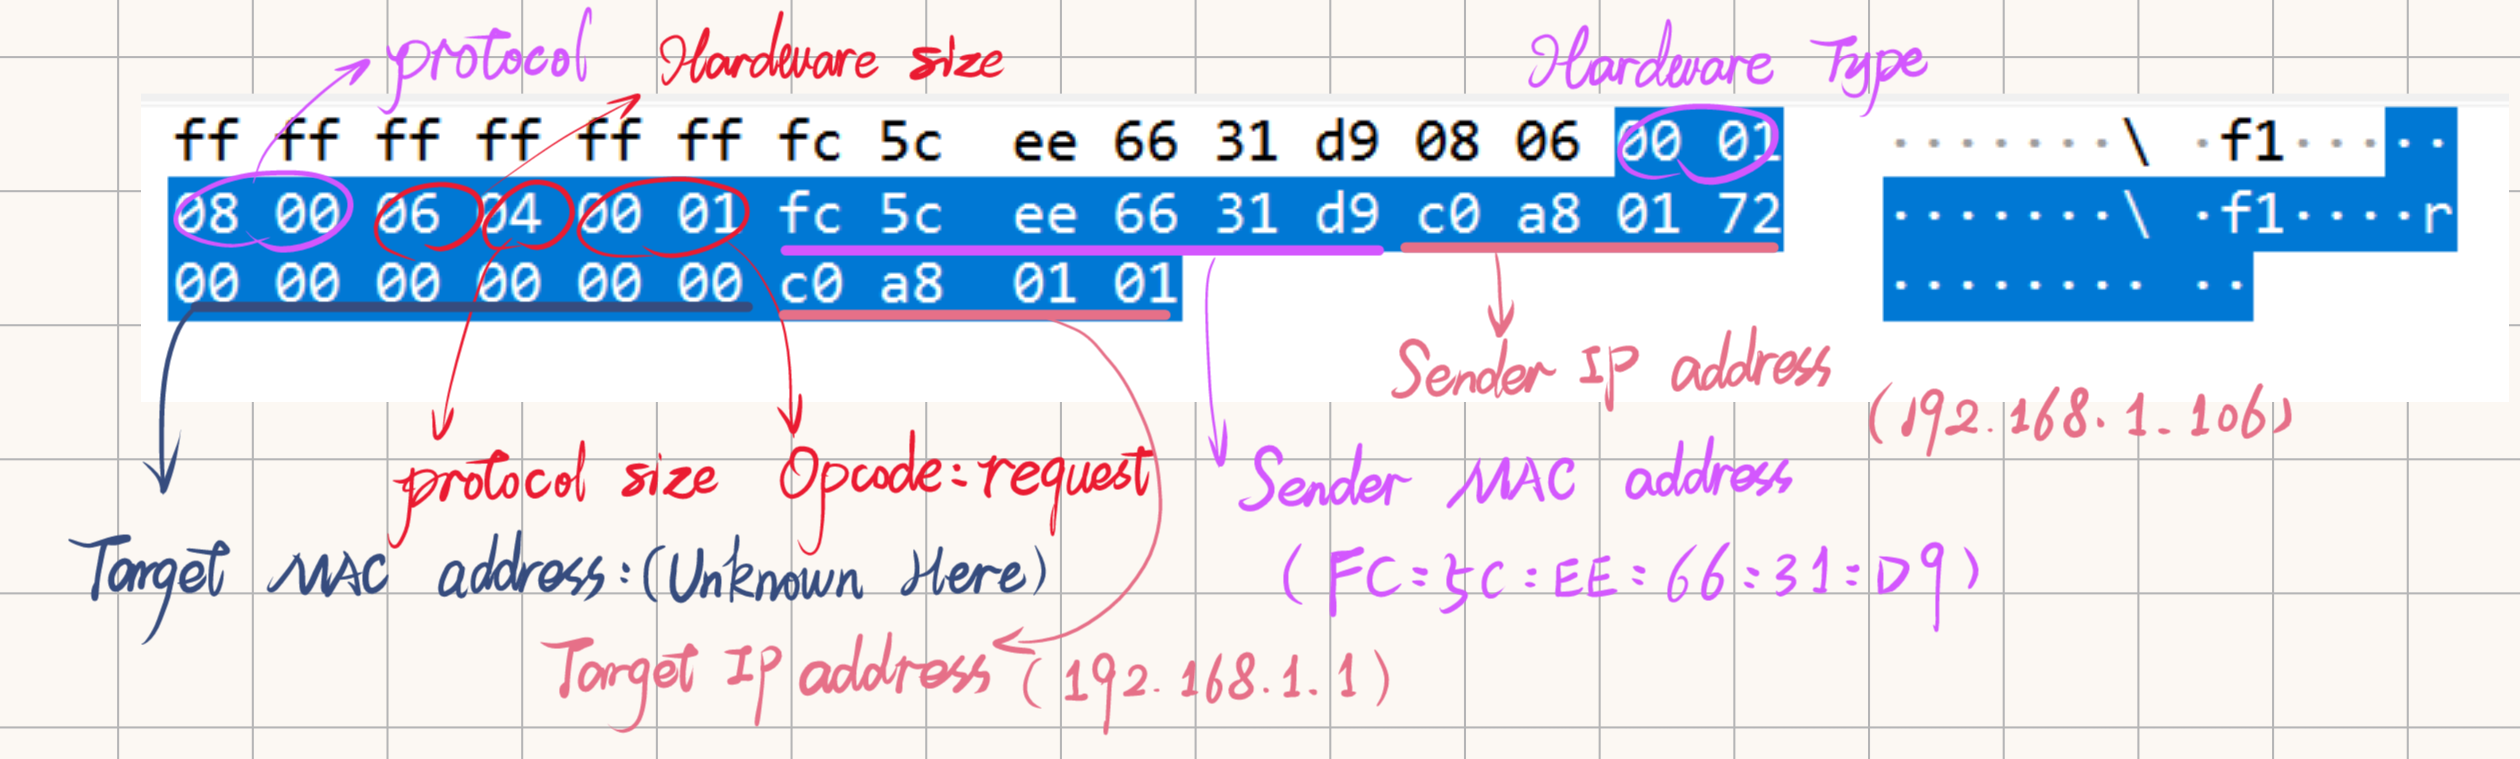
\includegraphics[width=0.8\textwidth]{lab4/draw.png}
    \caption{ARP 协议的结构}
\end{figure}

1、看以太网的头。
\begin{itemize}
    \item Destination: Broadcast (FF:FF:FF:FF:FF:FF),这是一个广播
    \item Source: FC:5C:EE:66:31:D9
    \item Type: 上一层协议是 ARP
\end{itemize}

2、看ARP的头
\begin{itemize}
    \item Hardware type:硬件类型,0x01 表示在以太网上传输
    \item Protocol type:上一层协议类型
    \item Hardware size:硬件长度
    \item Protocol size:协议长度
    \item Opcode: 操作类型,1为请求,2为应答
    \item Sender MAC address:fc:5c:ee:66:31:d9,发送方 MAC 地址
    \item Sender lP address:192.168.1.114,发送方IP
    \item Target MAC address:00:00:00:00:00:00,表示这是一个广播
    \item Target IP address:192.168.1.1,目标 IP
\end{itemize}

其实,这里就是先广播了自己的 MAC 地址和 IP 地址,并询问 IP 地址为 192.168.1.1 的路由
器的 MAC 地址是什么。当目标路由器收到 ARP 请求信息,并且自己的 IP 地址和请求信息
中的 IP 地址相匹配时,就会返回一个 ARP 回复

\subsubsection{ARP 的 Reply 帧}

接下来观察紧随其后的 Reply 帧的信息:

\begin{figure}[H]
    \centering
    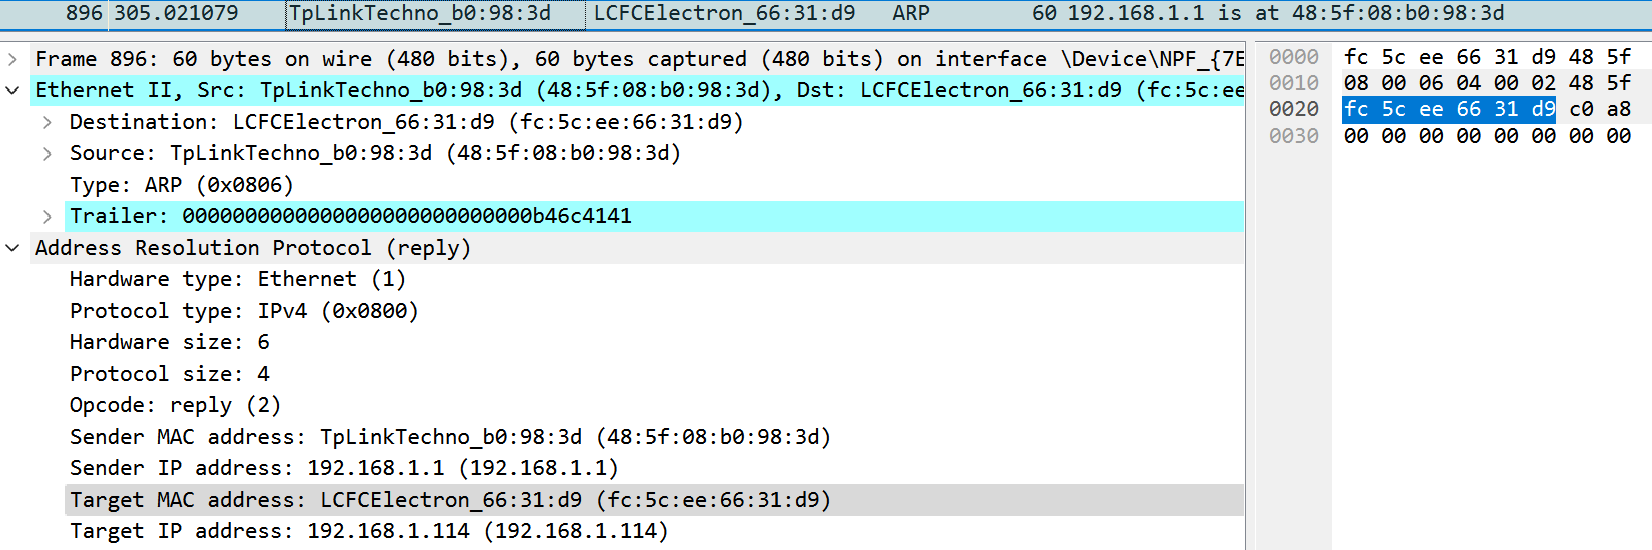
\includegraphics[width=0.65\textwidth]{lab4/reply.png}
    \caption{ARP Reply 帧}
\end{figure}

Reply 帧的每一个部分的字节长度和 Request 帧的结构相同。但在 Target MAC address
字节段不再全为 0,而是包含了目标 IP 地址路由器的 MAC 地址。除此之外,这里的 Opcode
字段也变成了 2,表示这是一个 Reply 帧。

\subsection{Step 3: ARP Request and Reply}

请求数据包应是广播的,而应答数据包是单播的。

注意到 Reply 帧中存在一个 Trailer 字段。它和传统的 Padding 字段有所不同。在以太网帧中,如果数据字段(Payload)长度小于 46 字节,以太网协议要求填充(Padding)字段,将帧的最小长度补充到 64 字节(含头部和 CRC 校验字段)。这是以太网规范的要求,用于确保帧的可靠性。

request消息是在发送之前就在本地被截获下来,因此没有padding字段。但reply消息是网卡处收到的字段,因此有padding字段。

\begin{figure}[H]
    \centering
    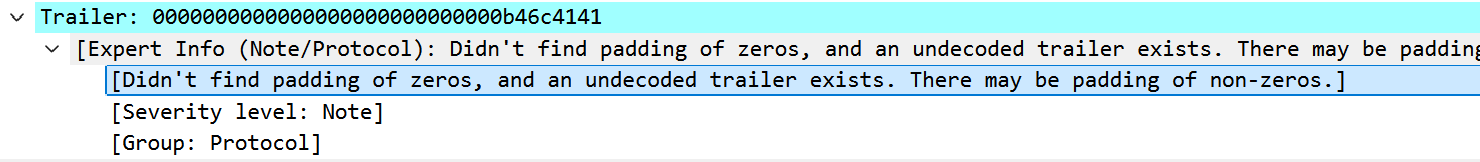
\includegraphics[width=0.65\textwidth]{lab4/nonzero.png}
    \caption{非零 Padding字段}
\end{figure}

\subsubsection{Trailer 的显示}
截图中提到:

\begin{lstlisting}
Didn't find padding of zeros, and an undecoded trailer exists.
\end{lstlisting}

它说明发现了一个未解析的 Trailer 字段,而不是传统的 Padding。

\subsubsection{Trailer 和 Padding 的区别}
\begin{itemize}[leftmargin=1.5em]
    \item \textbf{Padding:} 是为满足最小帧长的零填充。
    \item \textbf{Trailer:} 通常是附加信息(比如某些协议自定义的内容),不属于以太网的固定规范。
\end{itemize}

\subsubsection{绘制 Request 和 Reply 帧交互图}

根据上述的分析,可以按照要求画出带有 Sender 与 Receiver 的 IP / MAC 的 ARP 帧交流图。

\begin{figure}[H]
    \centering
    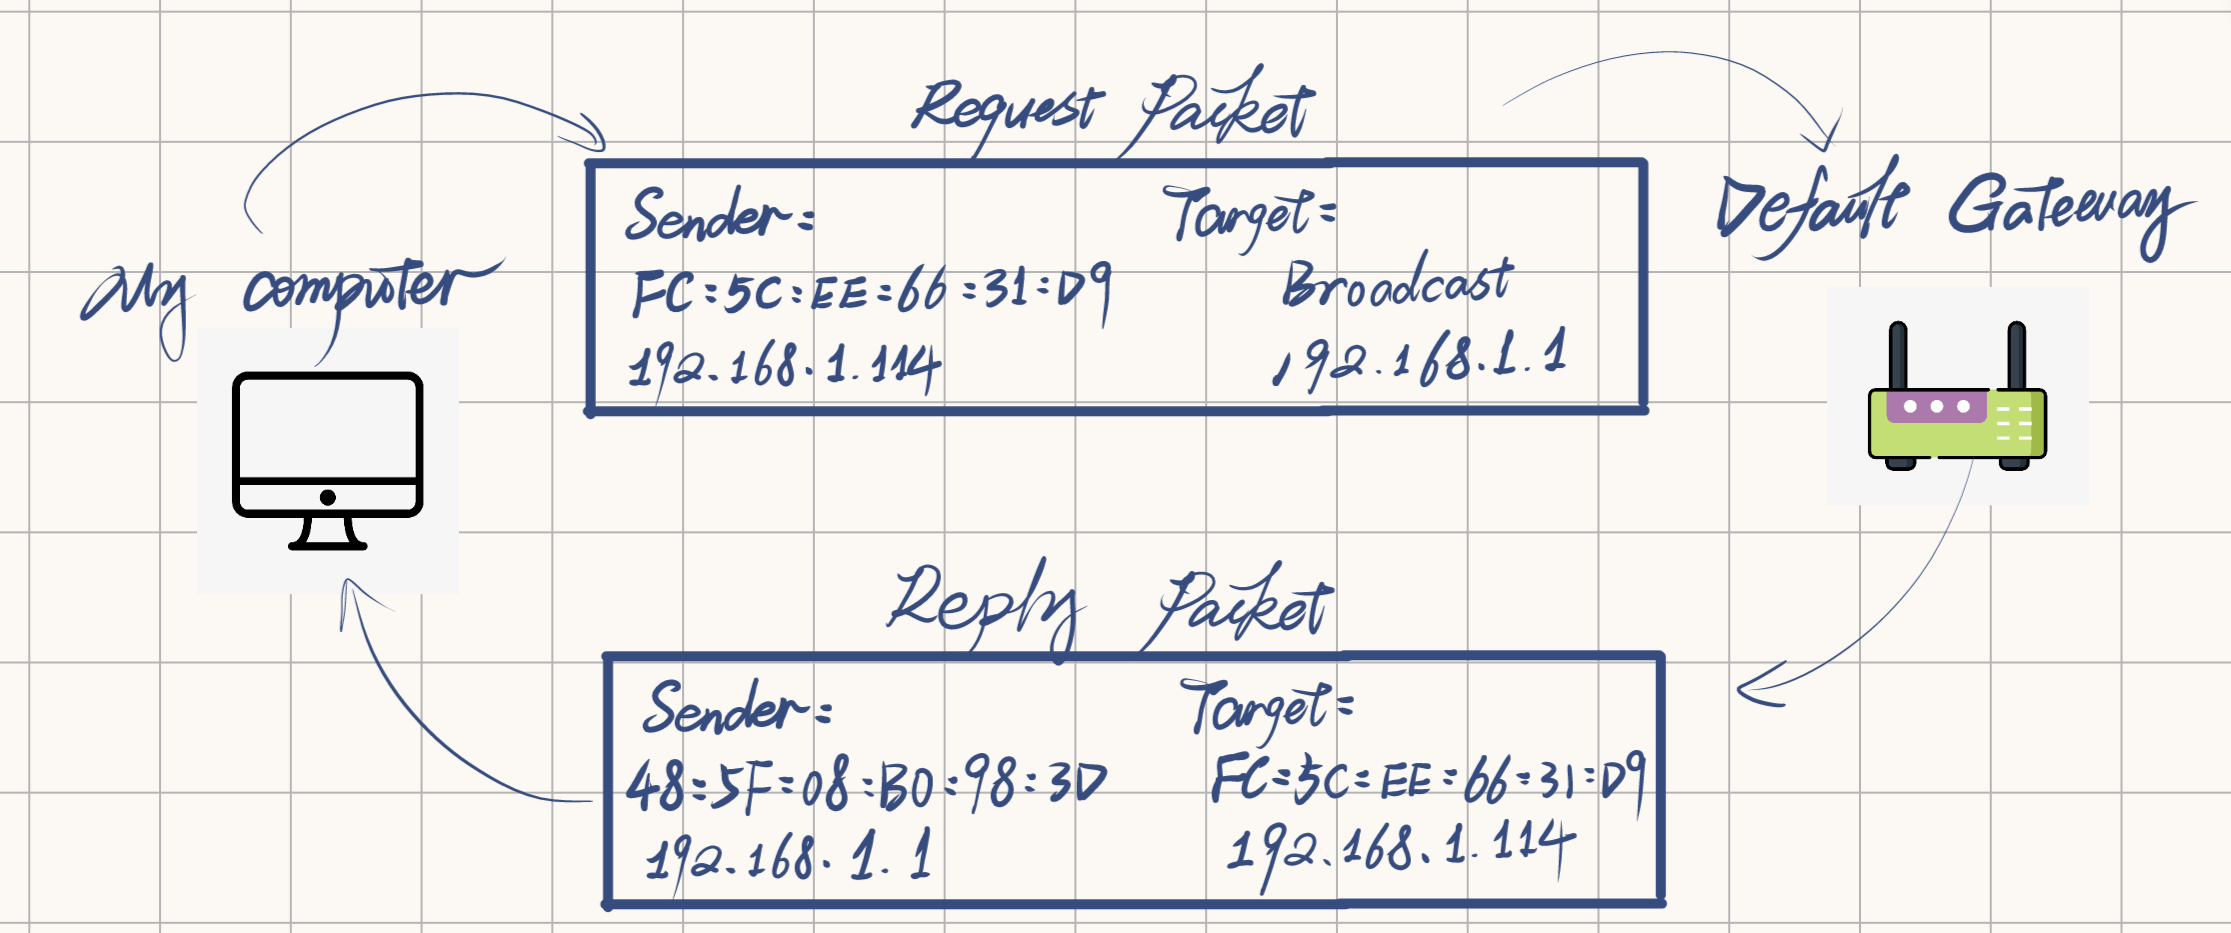
\includegraphics[width=0.8\textwidth]{lab4/draw2.png}
    \caption{Request 和 Reply 帧交互图}
\end{figure}

\subsection{课后思考题}

\subsubsection*{什么样的操作码是用来表示一个请求?应答呢?}
根据上面的分析和 Wireshark 抓包的结果,显而易见:请求操作码为1,回复操作码为2。

\subsubsection*{一个请求的ARP的报头有多大?应答呢?}
都是 28 字节。直接看 Wireshark 的抓包结果,点击 Address Resolution Protocol (request/reply) 查看即可。

\subsubsection*{对未知目标的MAC地址的请求是什么值?}
请求的目标MAC地址通常为全零,即00:00:00:00:00

\begin{figure}[H]
    \centering
    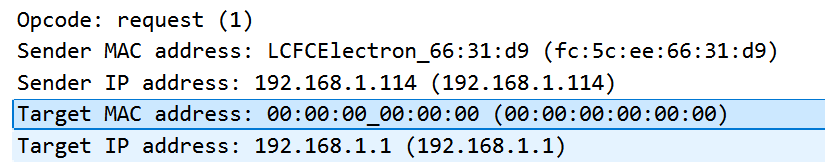
\includegraphics[width=0.8\textwidth]{lab4/q2.png}
    \caption{Question 3}
\end{figure}

\subsubsection*{什么以太网类型值说明ARP是更高一层的协议?}
ARP的以太网类型值为0x0806,也是从 Wireshark 的抓包结果中可以看到:

\begin{figure}[H]
    \centering
    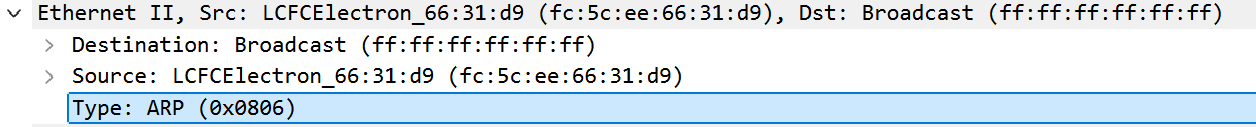
\includegraphics[width=0.8\textwidth]{lab4/q4.png}
    \caption{Question 4}
\end{figure}

\subsubsection*{ARP应答是广播吗?}
ARP应答通常不广播。它使用其以太网广播直接发送给目标。
也可以从最低字节的第一位看到这里的值为 0,表示为 unicast。

\begin{figure}[H]
    \centering
    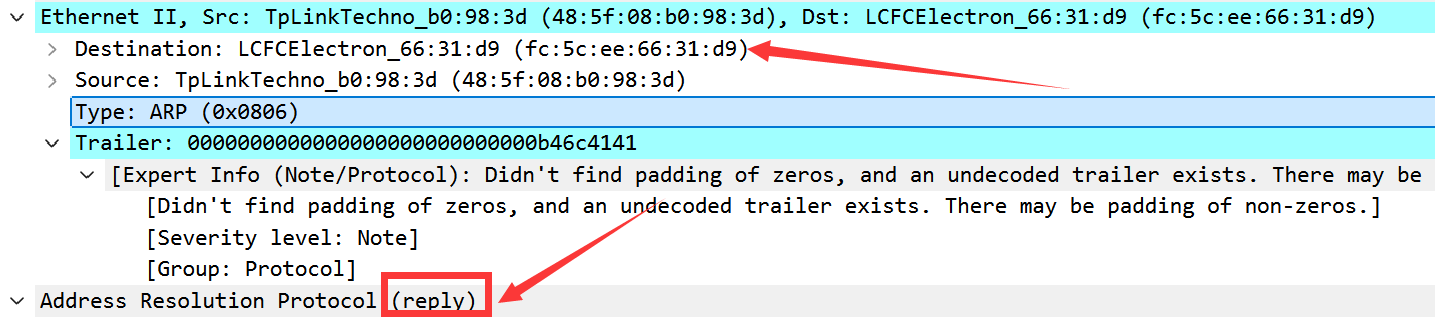
\includegraphics[width=0.8\textwidth]{lab4/qf.png}
    \caption{Question 5}
\end{figure}

\subsection{更多的 ARP 报文}

我们可以打开 lab4stu 中的 arp.pcap,查看更多的 ARP 报文:

\begin{figure}[H]
    \centering
    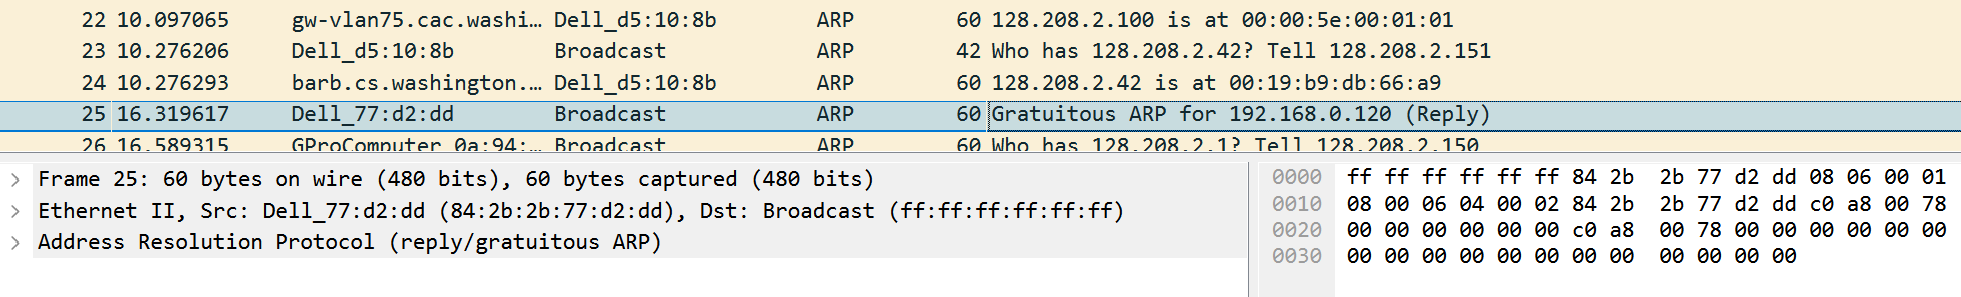
\includegraphics[width=0.8\textwidth]{lab4/more.png}
    \caption{More}
\end{figure}

在阅读 Info 字段时,可以看到除了网关和本机计算机之间的 arp 请求通信,还有局域网内许多其他计算机和本机的 ARP 请求(因为是广播形式,所以我们可以收到)。
当然,还有计算机发送的 arp 回复,告诉别的计算机我们的物理地址信息。

除此之外我们还可以看到有:

\begin{lstlisting}
    25	16.319617	Dell_77:d2:dd	Broadcast	ARP	60	Gratuitous ARP for 192.168.0.120 (Reply)
\end{lstlisting}

Gratuitous ARPs, (中文翻译为“无偿 ARP”或“任意 ARP”)是一种特殊的 ARP 报文。其主要特点和目的如下:

这类报文是自己的计算机发送的 arp 请求和答复,
目的是为了确保没有其他人正在使用相同的 IP 地
址。这类报文具有相同的发送方和目标 IP 地址,目的是检测 IP 冲突、通知其他设备更新 ARP 表或支持高可用性切换。它在网络配置和维护中起到了重要作用,虽然通常不会直接被用户感知,但在后台网络通信中广泛使用。



\section{实验结果总结}

通过本次 ARP 实验,我学会了在 Wireshark 中获得 ARP 数据包的方法,理解了 ARP(Address 
Resolution Protocol)的运作方式,并了解了在 ARP 报文信息的结构及每一部分代表的含义。

其实 ARP 协议只是提供了一种方法,根据目的主机的 IP 地址,获得其 MAC 地址。这便是地址解析的过程。
当然,我还通过运用 ipconfig、netstat、arp 等终端常用网络调试命令,进一步丰富了对网络的理解。

\section{附录}

\subsection*{参考资料}

\begin{itemize}
    \item 什么是 Gratuious ARPs:\href{https://blog.csdn.net/weixin_33754065/article/details/92784934}{\underline{https://blog.csdn.net/weixin\_33754065/article/details/92784934}}
\end{itemize}

\end{document}